\documentclass[conference]{IEEEtran}
\IEEEoverridecommandlockouts
% The preceding line is only needed to identify funding in the first footnote. If that is unneeded, please comment it out.
\usepackage{cite}
\usepackage{amsmath,amssymb,amsfonts}
\usepackage{algorithmic}
\usepackage{graphicx}
\usepackage{textcomp}
\usepackage{xcolor}
\def\BibTeX{{\rm B\kern-.05em{\sc i\kern-.025em b}\kern-.08em
		T\kern-.1667em\lower.7ex\hbox{E}\kern-.125emX}}

\begin{document}
	
	\title{Unraveling T Cell Receptor Specificity: An Integrated Approach to Sequence Analysis}
	
	\makeatletter
	\newcommand{\linebreakand}{%
	\end{@IEEEauthorhalign}
	\hfill\mbox{}\par
	\mbox{}\hfill\begin{@IEEEauthorhalign}
	}
	\makeatother
	
	\author{\IEEEauthorblockN{Shalomi Fernandes}
		\IEEEauthorblockA{\textit{Department of Engineering and Mathematics} \\
			\textit
            University of Bristol \\
			Bristol, United Kingdom \\
			mh23950@bristol.ac.uk}
		\and
		\IEEEauthorblockN{Fangnan Wei}
		\IEEEauthorblockA{\textit{Department of Engineering and Mathematics} \\
			\textit
            University of Bristol \\
			Bristol, United Kingdom \\
			tj23631@bristol.ac.uk}
		\linebreakand %
		\IEEEauthorblockN{Jiadong Xu}
		\IEEEauthorblockA{\textit{Department of Engineering and Mathematics} \\
			\textit
            University of Bristol \\
			Bristol, United Kingdom \\
			jiadong.xu.2021@bristol.ac.uk}
		\and
		\IEEEauthorblockN{Jiahui Liu}
		\IEEEauthorblockA{\textit{Department of Engineering and Mathematics} \\
			\textit
            University of Bristol \\
			Bristol, United Kingdom \\
			ye23356@bristol.ac.uk}
	}
	
	\maketitle
	
	\begin{abstract}
		This study utilizes machine learning techniques to predict the specificity of T cell receptors (TCRs), which play a key role in the immune system's response to pathogens and cancer cells. Our research focuses on the broad diversity of TCR sequences in the VDJdb dataset to understand their interactions with specific epitopes. We have developed a method that includes the preprocessing of TCR sequence data, we have used techniques such as Encoding, computational distance matrix, classification, dimensionality reduction, clustering techniques to process the VDJdb dataset, and we have also built an algorithm aimed at predicting antigen specificity. Our innovative computational approach is expected to overcome the limitations of current empirical approaches and significantly improve the effectiveness of immunotherapies and personalized medicine. This article presents the results of our research on the predictive accuracy of these methods and discusses potential improvements and future research directions.
	\end{abstract}
	
	\section{Introduction}
	This study aims to predict the specificity of T cell receptors (TCRs) by machine learning techniques. TCRs are a key component of the immune system, which is able to recognize and respond to antigens presented by pathogens or cancerous cells through a highly variable molecular structure. This diversity is primarily generated through the recombination of variable (V), diversity (D), and junction (J) gene fragments, allowing TCRs to bind to a variety of peptides presented by major histocompatibility complex (MHC) molecules. However, due to the complexity and high variability of peptide-MHC-TCR interactions, the use of sequence data to predict the specificity of TCRs remains a challenge. Most of the existing traditional methods rely on empirical data, which often cannot accurately capture the nuances of antigen recognition. Therefore, this research aims to develop an innovative computational method that can more accurately simulate and predict TCR behavior through in-depth analysis of the vast TCR sequence data in the VDJdb database, which is expected to drive the development of personalized medicine and immunotherapy.
	
	Predicting TCR specificity is critical for advancing immunotherapies and designing targeted therapies. The project involves preprocessing TCR sequence data, encoding, calculating distances, classification, clustering, dimensionality reduction techniques, and developing algorithms for predicting antigen specificity. We focus on extracting meaningful patterns from TCR sequences using dimensionality reduction and clustering techniques, with the aim of developing robust predictive models. Our approach aims not only to enhance the understanding of TCR-antigen interactions, but also to advance personalized medicine by facilitating the development of more effective immunotherapies.By combining computational methods with immunological insights, our research explores new areas of immunoinformatics, paving the way for breakthroughs in the understanding and therapeutic utilization of the immune system. This research has great potential to enhance the efficacy of personalized medicine and immunotherapy, and to address the limitations of current empirical approaches through innovative computational methods.
	
	\section{Literature Review}
	
	"GIANA allows computationally-efficient TCR clustering and multi-disease repertoire classification by isometric transformation" \cite{b1} introduces a TCR alignment algorithm GIANA(Geometric Isometry-based TCR AligNment Algorithm) based on geometric isometric transformation, a new computational tool designed to improve the efficiency and accuracy of T cell receptors. GIANA not only improves calculation speed (600 times faster than TCRdist without sacrificing accuracy), but also facilitates fast queries of large reference queues. It successfully identified novel disease-associated TCRs and classified unseen samples in a variety of diseases, including cancer, infectious diseases, and autoimmune diseases.
    \\

    "T cell receptor sequence clustering and antigen specificity" \cite{b2} describes clustering techniques for classifying TCR sequences based on their biological similarity and antigen specificity. Technological advances have made TCR sequencing data widely available, and there is increasing interest in understanding TCR-epitope interactions to predict disease outcome, track treatment efficacy, and stratify patients for treatment. This review discusses several sequencing-based methods, including sequence alignment, analysis of short TCR motifs, and the use of various computational tools to predict TCR binding based on structural and sequence data, highlighting the challenges of these methods, such as the need for large data set and the complexity of predicting protein interactions based on sequence data alone. The paper also explores future directions for improving TCR sequence analysis, showing that integrating more sophisticated machine learning models and structural data can improve the predictive accuracy of these methods.
    \\
	
	"TCR meta-clonotypes for biomarker discovery with tcrdist3 enabled identification of public, HLA-restricted clusters of SARS-CoV-2 TCRs" \cite{b3} introduces a new framework to classify biochemically similar TCRs into "meta-clonotypes". Researchers used the newly developed open source software package tcrdist3 to analyze TCR data from COVID-19 patients to create and quantify meta-clonotypes, providing a more powerful tool for identifying disease-associated TCR patterns. Application of this method identified 1,831 public TCR metaclonotypes associated with SARS-CoV-2, and significant HLA restriction was observed. Meta-clonotypes were more frequently detected in the TCR repertoires of patients with specific HLA genotypes than exact amino acid matches.
	
	\section{Methodology}
	In this study, the data is preprocessed, encoded, distance calculation of TCR sequences is done followed by dimensionality reduction, clustering, classification, and analysis of predictions. The encoding methods used in this article is One-Hot, BLOSUM 62 and GIANA Encoding. The distance calculation methods used in this article are TCRDist, GIANA and Levenshtein. The dimensionality reduction methods used in this article are PCA, t-SNE and UMAP. The clustering methods used in this article are Agglomerative Hierarchical clustering and DBSCAN. The classification method useds in this article are Logistic Regression, SVM, and RandomForestClassifier.
	
	
	\subsection{Pre-Processing}
	In this study, the data preparation process involved several key steps to ensure the cleanliness, relevance, and structured organization of the dataset. This included loading the TCR sequence data, followed by comprehensive data cleaning procedures to handle missing values and remove duplicates. Relevant features were carefully selected based on their significance to the analysis goals, while new features were engineered to enhance the model's ability to discern meaningful patterns. Additionally, normalization or standardization techniques were applied to bring features to a comparable scale, and dimensionality reduction methods like PCA, t-SNE, or UMAP were employed to visualize complex datasets and streamline subsequent analyses. Overall, these steps were pivotal in readying the dataset for further exploration and modeling. These steps are discussed in detail in the Methodology Section.
	
	\subsection{Encoding Methods:}
	\subsubsection{One-Hot Encoding} \
	
	One-hot encoding\cite{b2} is a technique for representing categorical variables as binary vectors. In this encoding, the value of each variable is represented as a vector of length equal to the number of possible values, with only one element being 1 (representing the category to which the variable belongs) and all other elements being 0. In this work, we defined a function for one-hot encoding, which takes two parameters: the sequence to be encoded and a list of all possible amino acids. The function creates a two-dimensional array with the number of rows equal to the length of the sequence and the number of columns equal to the number of types of amino acids, it iterates through each amino acid in the sequence, and sets the value of the corresponding position to 1 if the amino acid is in a given list of amino acids, indicating that the amino acid appears, otherwise it is 0.
    \\

    Using a one-hot representation to encode TCR sequences has several limitations in downstream analysis. One major limitation is the inability to capture the sequential nature of amino acids, resulting in a loss of important structural and functional information. Additionally, one-hot encoding can lead to high-dimensional sparse representations, especially for TCR sequences with variable lengths of CDR3 regions, making it challenging to analyze and compare sequences effectively. To overcome these limitations, a possible approach is to incorporate information about the CDR3 length distribution. 
    \\
	
	\subsubsection{BLOSUM 62 ENCODING} \

    Since one-hot encoding represents amino acids as binary vectors without considering their biochemical properties or evolutionary relationships, it may not capture the nuanced differences between sequences effectively. In contrast, we utilized the BLOSUM62 (BLOcks SUbstitution Matrix 62) for distance matrix calculation. BLOSUM62 assigns scores to pairs of amino acids based on their observed frequencies in related proteins, capturing both the similarities and differences between sequences in a biologically meaningful way. This approach provides a more accurate representation of sequence similarity and is better suited for our analysis compared to one-hot encoding.
    \\
    
	BLOSUM 62\cite{b2} encoding is a protein sequence encoding method that is based on the score of the BLOSUM (Blocks Substitution Matrix) substitution matrix. The BLOSUM 62 substitution matrix is derived from statistical analysis of a large number of known protein sequences to assess the similarity between two amino acids. In the BLOSUM 62 encoding, each amino acid is mapped to a vector whose length is equal to the number of rows of the substitution matrix. Each element in the vector represents the similarity score of that amino acid to the corresponding row in the substitution matrix.
    \\
	
	\subsubsection{GIANA ENCODING} \
	
	GIANA Encoding\cite{b2} converts TCR sequences into numerical representations of fixed dimensions. The core idea of GIANA Encoding is to use Autoencoder to learn the low-dimensional representation of TCR sequences. The Autoencoder consists of an encoder and a decoder that can learn a compressed representation of the data. In GIANA Encoding, the encoder is responsible for mapping the TCR sequence to the low-dimensional space, while the decoder is responsible for mapping the low-dimensional representation back to the original TCR sequence space.
    \\
	
	\subsection{Distance Calculation Methods:}
	
	\subsubsection{TCRDist} \
	 We employed TCRdist, a specialized tool for computing pairwise distances between T-cell receptor sequences. We divided the dataset into six subsets: human alpha, human beta, combined human alpha-beta, mouse alpha, mouse beta, and combined mouse alpha-beta as shown in Fig.1. which shows the subdivision of data for TCR Distance Matrix Calculation. Each subset was processed to calculate the TCR distance matrix for both alpha and beta chains. The distance matrices were essential for quantifying the similarity between TCR sequences, which is a crucial step for further analysis such as clustering and dimensionality reduction. 

    \begin{figure}[h]
		    \centering
		    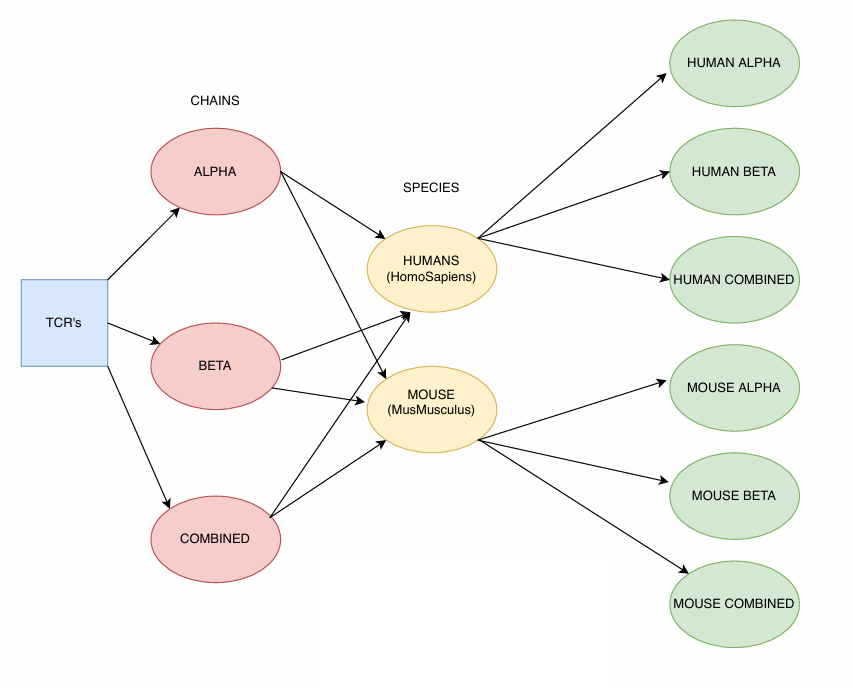
\includegraphics[width=0.5\linewidth]{fig1.png}
		    \caption{Subdivision of TCR Distance Matrix Calculation}
		    \label{fig:enter-label}
		\end{figure}
 
	TCRDist\cite{b2}\cite{b3} is a toolkit for calculating TCR distances, which can be calculated based on their sequence characteristics (e.g., CDR3 sequences) and possibly other information (e.g., expression patterns of TCRs).For a given set of TCR sequences, the distances between all possible pairs are calculated, and the results are formed into a distance matrix, each element in the matrix represents the distance or similarity between the pairs, and once the distance matrix is calculated, visualization tools can be used to show the similarity or difference between the TCRs.
    \\
	
	\subsubsection{Levenshtein} \
	
	Levenshtein distance is a measure of how similar two strings are. Levenshtein distance is calculated by performing a series of insert, delete, and replace operations on one string to make it equal to another, and it represents the minimum number of edit operations required to convert one string to another.
	
	This article creates a function levenshtein\_distance\_matrix which is used to calculate the Levenshtein distance between a set of sequences. The function first calculates the length of the list of input sequences and creates an all-zero square matrix of size for the number of input sequences. Then, iterate over each pair of sequences in the sequence list, call the levenshtein\_distance function to calculate the edit distance between them, and fill in the result to the corresponding position of the all-zero square.
	\\
    \subsection{Dimensionality Reduction Method:}
	\subsubsection{UMAP} \
	
	UMAP (\emph{Uniform Manifold Approximation and Projection}) is a nonlinear dimensionality reduction algorithm, similar to t-SNE, but with faster computation speed and better ability to maintain the global structure than t-SNE.
	
	For dimensionality reduction, we utilized the UMAP (Uniform Manifold Approximation and Projection) algorithm to project the high-dimensional TCR data into a two-dimensional space. This transformation was applied separately to the encoded data from each of the six subsets. The UMAP plots were then generated to visually represent the clustering of TCR sequences based on their specificity to different epitopes, allowing us to observe the potential groupings of similar TCR sequences.
      
    \subsection{Clustering Methods}
	\subsubsection{Agglomerative Hierarchical Clustering} \
	
	Agglomerative Hierarchical Clustering\cite{b4} is a clustering algorithm that gradually merges data points into clusters, and represents the similarity relationship between data points through a tree-like structure. Agglomerative Hierarchical Clustering takes the distance between data points as a measure of similarity, and then gradually merges the data points into different clusters based on preset parameters (number of clusters, distance metric, and linking method).
    \\
	
	Mathematical Description:
	
	Start by treating each data point as a single cluster. Let $C = \{C_1, C_2, \ldots, C_N\}$ be the initial set of clusters where each $C_i$ contains a single data point. Define a similarity measure (or distance measure) $d(C_i, C_j)$ between two clusters $C_i$ and $C_j$.
	
	Find the closest (most similar) pair of clusters and merge them into a single cluster.Mathematically, if $C_i$ and $C_j$ are the closest pair, they are merged to form a new cluster $C_k$.
	
	After merging $C_i$ and $C_j$, update the distance matrix to reflect the distances of the new cluster $C_k$ to all existing clusters. 
	\begin{itemize}
		\item \textbf{Single Linkage}:
		
		$d(C_k, C_x) = \min(d(C_i, C_x), d(C_j, C_x))$
		\item \textbf{Complete Linkage}: 
		
		$d(C_k, C_x) = \max(d(C_i, C_x), d(C_j, C_x))$
		\item \textbf{Average Linkage}: 
		
		$d(C_k, C_x) = \frac{d(C_i, C_x) + d(C_j, C_x)}{2}$
		\item \textbf{Ward's Method}: Merge the pair of clusters that results in the minimum increase in total within-cluster variance after merging.
	\end{itemize}
	
	Repeat these steps until all data points are clustered into a single cluster of size $N$. As clusters are merged, a tree-like diagram called a dendrogram is created to record the sequences of merges. This dendrogram illustrates how each cluster is composed by branching out to its constituent elements.
    \\
	
	In this work, the number of clusters was set to 5, and the similarity between the clustering results and the real labels and the clustering quality were evaluated by using the Adjusted Rand Index and Silhouette Score. The Adjusted Rand Index measures how similar the clustering results are to the real labels, with values between -1 and 1, with closer to 1 indicating that the clustering results are more similar to the real labels. The Silhouette Score measures the clustering closeness of each sample and ranges from -1 to 1, with closer to 1 indicating better clustering results.
	\\
 
	\subsubsection{DBSCAN} \
	
	DBSCAN is a popular clustering algorithm that identifies clusters of different shapes and sizes in a dataset, unlike methods such as K-means, DBSCAN does not require pre-specifying the number of clusters to be identified.
	
	For each point in the dataset, DBSCAN calculates how many points are within that eps (the maximum distance between two points, where one point is considered to be within the neighborhood of the other point, and the smaller the value, the more clustering) distance. If the count exceeds min\_samples (the minimum number of points required to form a dense area, higher values usually result in more points being treated as noise), then the point is marked as a core point; Starting from a core point, DBSCAN recursively finds all the points that are dense from that point and assigns them to the same cluster; Neither the core nor any core point where the direct density is reachable is marked as noise.
    \\
	
	In this study, the DBSCAN algorithm is used to cluster the data in the distance matrix, and the eps parameter (neighborhood radius) and min\_samples parameter (minimum number of samples) are set, which determine the clustering results, which include the clustering label of each sample point and the label of the noise point. Finally, the contour coefficient of the clustering result is calculated using silhouette\_score. The contour coefficient is an index to measure the degree of tightness and separation of clustering results, and the value range is between [-1, 1], and the closer the value is to 1, the better the clustering result.
	
	In this study, there are three values worthy of our attention, namely purity fraction, purity fraction and NMI\cite{b1}.
	\begin{itemize}
		\item Purity Fraction is defined as the percentage of pure clusters in the clustering output, where a pure cluster is one where all the TCRs are specific to the most common epitope in that cluster. 
		\item Purity Retention refers to the proportion of TCRs in all the pure clusters divided by the total number of TCRs in the test set. It provides an indication of how many TCRs in the dataset end up in pure clusters. 
		\item NMI is used to measure the mutual information between TCR clusters and epitope specificity, normalized by the sum of their individual entropies. It provides a standardized measure of the degree of association between the clustering of TCR sequences and their antigen specificities.
	\end{itemize}
 
	\subsection{Model Building (Classification Models):}
	\subsubsection{Data Preparation} \
    The dataset contained several columns that were not necessary for building the predictive models. By retaining key features the dataset is refined to include only those attributes that provide essential information about the TCRs and their interactions with antigens. Epitopes with fewer than 10 occurrences are considered insufficient for reliable modeling and were thus filtered out. This focuses the dataset on more common epitopes, which improves the model's ability to learn relevant patterns and make accurate predictions.
    \\
    
    We Calculated the length of each CDR3 sequence and retaining those within a practical range (10 to 20 amino acids), as very short or very long sequences might represent sequencing errors or unusual variations that could skew the model training. We counted the occurrences of each species and filtered to include only those species with sufficient representation (over 1000 occurrences), thus focusing on more common contexts in the training data. Further, we filtered the dataset to exclude rows where complex.id is 0. This step removed entries that did not meet certain criteria essential for our analysis, such as incomplete data entries or placeholders that do not correspond to actual TCR sequences. By doing this, we ensured that the dataset consists only of meaningful and relevant entries, enhancing the quality of our training data.
	\\
 
    This model first uses a combination of Label Encoding and Binary Encoding to encode features like 'gene', 'species', 'epitope','mhc.a', 'mhc.b', 'v.segm' and 'j.segm' and 'mhc.class'. Next, using a function GIANA\_encoder\_pd, the CDR3 sequence is encoded into a vector representation, first traversing each amino acid sequence, for each sequence, removing the C and J segments at the beginning, and the F segment at the end, encoding the sequence using a predefined M6 matrix. For each row, the encoded CDR3 sequence and the normalized eigenvalues are first concatenated, and then they are combined into a single array. Finally, the resulting array contains the encoded CDR3 sequence and all the normalized eigenvalues, so that each row represents a complete sample eigenvector.
    \\
    \subsubsection{Data Selection} \
    We made a decision to focus exclusively on Human Species (Homo Sapiens) for model building and predictions due to the significantly larger volume of data available—51,535 entries for humans compared to just 4,173 for mice (Mus Musculus). This stark disparity allows for a more robust and generalizable model for humans, where the richer dataset ensures more reliable predictive performance. Additionally, focusing on human data aligns with the primary goal of applying findings directly to human medicine, avoiding the risks of undertraining and overfitting associated with the limited mouse data. This approach not only makes efficient use of the extensive human data but also enhances the clinical relevance of the predictions. 
    \\
    
    We subdivided the dataset to obtain the alpha and the beta chains and performed model evaluations. Each chain potentially interacts differently with antigens, influencing the specificity and strength of immune responses. By analyzing them separately, it's possible to isolate and understand the unique contributions of each chain to antigen recognition. This approach allows for a more nuanced analysis of TCR behavior, providing insights that could be obscured in a combined model. Moreover, separate evaluations enable the identification of chain-specific patterns, which are crucial for developing targeted therapeutic strategies and enhancing the accuracy of predictive immunological models.
    \\

    \subsubsection{Logistic Regression (Baseline Model)} \
    The baseline model for predicting T-cell receptor (TCR) specificity utilizes logistic regression, a choice driven by the model's robustness and simplicity for binary classification tasks. During training, the dataset was split into training and testing sets to validate the model's performance on unseen data. The primary evaluation metric selected was the F1 score, due to the imbalanced nature of the dataset where accuracy alone could be misleading. This was particularly important given the variability in epitope representation within the dataset.
    \\

    \subsubsection{SVM Model)} \
    In this project, the Support Vector Machine (SVM) classifier was employed as another method for building predictive models to understand antigen specificity from T-cell receptor (TCR) sequences. The SVM was chosen for its effectiveness in high-dimensional spaces, as it excels in finding the optimal hyperplane that maximizes the margin between different classes. Specifically, the linear kernel was utilized to handle the linearly separable aspects of the data. The training process involved splitting the dataset into training and testing sets to both train the SVM and validate its performance on unseen data. This method provided a systematic approach to model antigen recognition patterns in an attempt to predict responses based on the molecular features of the TCR sequences.
    \\
    
    \subsubsection{Random Forest Classifier Model)} \
    The Random Forest classifier demonstrates a marked improvement over the logistic regression and SVM models primarily due to its ensemble learning approach, which integrates multiple decision trees to produce a more stable and accurate prediction by averaging the results. This method effectively reduces the variance and overfitting problems often seen in single decision tree models, leading to enhanced generalizability across diverse datasets. Specifically, the Random Forest model exhibited higher weighted average F1 scores, indicating superior performance in balancing precision and recall across various classes within the imbalanced dataset.
    \\

    \subsection{Hyperparameter Tuning on the Random Forest Model}
	Hyperparameter tuning of the Random Forest model significantly enhanced its performance for both Alpha and Beta chains, illustrating the importance of optimizing model parameters in handling complex immunological datasets. The tuning was conducted using RandomizedSearchCV, where parameters such as the number of estimators, maximum features, maximum depth, minimum samples split, minimum samples leaf, and the use of bootstrap were varied across a predefined grid. This process was repeated across 10 iterations with 3-fold cross-validation to maximize robustness and effectiveness.
    \\
    
    These traits make Random Forest particularly effective in handling the complex patterns and intricacies of antigen specificity prediction, where robustness against diverse and skewed data distributions is crucial. This enhanced capability to deliver more reliable and consistent predictions across a wider range of T-cell receptor specificities underlines why Random Forest is a preferable choice over the simpler logistic regression and the linear-bound SVM in this context. 

    
    
	\subsection{Figures and Tables}
	\paragraph{Positioning Figures and Tables} Place figures and tables at the top and 
	bottom of columns. Avoid placing them in the middle of columns. Large 
	figures and tables may span across both columns. Figure captions should be 
	below the figures; table heads should appear above the tables. Insert 
	figures and tables after they are cited in the text. Use the abbreviation 
	``Fig.~\ref{fig}'', even at the beginning of a sentence.
	
	\begin{table}[htbp]
		\caption{Table Type Styles}
		\begin{center}
			\begin{tabular}{|c|c|c|c|}
				\hline
				\textbf{Table}&\multicolumn{3}{|c|}{\textbf{Table Column Head}} \\
				\cline{2-4} 
				\textbf{Head} & \textbf{\textit{Table column subhead}}& \textbf{\textit{Subhead}}& \textbf{\textit{Subhead}} \\
				\hline
				copy& More table copy$^{\mathrm{a}}$& &  \\
				\hline
				\multicolumn{4}{l}{$^{\mathrm{a}}$Sample of a Table footnote.}
			\end{tabular}
			\label{tab1}
		\end{center}
	\end{table}
    
	
	
	Figure Labels: Use 8 point Times New Roman for Figure labels. Use words 
	rather than symbols or abbreviations when writing Figure axis labels to 
	avoid confusing the reader. As an example, write the quantity 
	``Magnetization'', or ``Magnetization, M'', not just ``M''. If including 
	units in the label, present them within parentheses. Do not label axes only 
	with units. In the example, write ``Magnetization (A/m)'' or ``Magnetization 
	\{A[m(1)]\}'', not just ``A/m''. Do not label axes with a ratio of 
	quantities and units. For example, write ``Temperature (K)'', not 
	``Temperature/K''.
	
	
	
	\section{Results and Discussion}
	{\color{blue}Reporting on the experiments with discussion on insights. Technical challenges are to be discussed here too.}

    \subsubsection{Logistic Regression (Baseline Model)} \

    Model evaluation revealed that while the overall accuracy appeared high at approximately 87.5\% for the alpha chains and 87.75\% for the beta chains, the F1 scores for many classes were very low, indicating poor performance in correctly classifying many specific epitopes. This discrepancy between high accuracy and low F1 scores highlighted the challenges of working with imbalanced datasets and underscored the necessity of choosing appropriate metrics for performance evaluation. The classification report showed substantial variability in precision, recall, and F1 scores across different classes, with many classes showing zero values in these metrics, suggesting that the model struggled with minority classes. This outcome stresses the importance of further model adjustments and potentially exploring more complex models or resampling techniques to better handle class imbalance and improve the model's ability to generalize across less frequent classes.
    \\
	
	\subsubsection{SVM} \
	The SVM classifier, using a linear kernel, achieved an accuracy of approximately 87.51\% for the alpha chains and 89\% for the beta chains, which closely aligns with the logistic regression model, suggesting similar overall predictive performance across the dataset. However, a deeper look at the F1 scores from the classification report indicates that the SVM struggles with several classes, achieving zero F1 scores for many, highlighting the challenges of classifying minority classes within an imbalanced dataset. Despite these struggles, the SVM has shown strengths in certain areas, achieving high F1 scores (up to 1.0) in specific classes where logistic regression may not perform as effectively. This ability to distinctly manage certain data subsets where SVM's optimization excels indicates a more nuanced performance, especially in precision and recall balance, evidenced by a weighted average F1 score of 0.88 both both alpha and beta chains. While SVM's accuracy parallels that of logistic regression, its superior F1 scores in particular classes underline its potential for providing more reliable predictions for specific TCR specificities, which is crucial for applications in clinical and immunological contexts.
    \\

    \subsubsection{Random Forest Classifier} \
	
	The Random Forest classifier, applied separately to Alpha and Beta chains, demonstrates distinctive performance metrics with notable strengths and limitations. For both chains, the model achieves a high overall accuracy, reaching around 90\% and 92\% respectively, indicating strong general predictive capabilities across the dataset. However, a deeper analysis using the F1 scores reveals a mixed performance in classifying individual epitopes. Several classes achieve low to zero F1 scores, reflecting the classifier's struggle with minority classes within the imbalanced dataset. Conversely, certain classes see substantial F1 scores, showcasing the model's potential in accurately predicting specific classes.
    \\

    This mixed outcome underscores the Random Forest model's ability to manage complex data through its ensemble approach, effectively capturing multiple decision paths and reducing variance compared to single estimators like logistic regression. The high weighted average F1 scores (0.91 for Alpha and 0.92 for Beta chains) further highlight its capability to balance precision and recall across various classes, making it a robust choice for tackling the intricacies of TCR specificity. The model's performance suggests that while it excels in overall accuracy and handling specific classes well, there remains a need for improved strategies or additional model tuning to enhance its precision across all classes.
    \\

    \begin{figure}[h]
		    \centering
            \includegraphics[width=7cm]{fig2.png}
		    %\includegraphics[width=0.5\linewidth]{fig2.png}
		    \caption{Comparison of F1 scores across different models for the Alpha and Beta Chains}
		    \end{figure}
      
    \subsection{Hyperparameter Tuning on the Random Forest Model}

    The outcomes of the tuning revealed substantial improvements. For the Alpha chain, the optimal set of hyperparameters increased the weighted average F1 score to 0.91, up from pre-tuning scores, indicating a more precise balance between recall and precision in predicting various classes. Similarly, the Beta chain also showed improved performance with the same weighted average F1 score of 0.91. These enhancements suggest that the tuned Random Forest model is more adept at managing the skewed distributions and diversity of the dataset, leading to more reliable predictions. This improvement is particularly significant in a clinical setting, where accurate and dependable model predictions are crucial for developing targeted immunotherapies based on T-cell receptor specificities.
	
	\section{Further Work and Improvement}
	{\color{blue}Explore what can be done further based on the discussed insights and ways to improve.}
    
	
	\section{Conclusion}
	{\color{blue}A brief summary of the key insights in your report.}
	
	\begin{thebibliography}{00}
		%\bibitem{b1} H. Huang, C. Wang, F. Rubelt, et al., Analyzing the Mycobacterium tuberculosis immune response by T-cell receptor clustering with GLIPH2 and genome-wide antigen screening, Nature Biotechnology, vol. 38, no. 10, pp. 1194-1202, 2020.
		
		\bibitem{b1} H. Zhang, X. Zhan, and B. Li, "GIANA allows computationally-efficient TCR clustering and multi-disease repertoire classification by isometric transformation," Nature Communications, vol. 12, no. 1, pp. 4699, 2021.
		
		\bibitem{b2} M. Vujovic, K. F. Degn, F. I. Marin, et al., "T cell receptor sequence clustering and antigen specificity," \textit{Computational and Structural Biotechnology Journal}, vol. 18, pp. 2166-2173, 2020.
		
		\bibitem{b3} K. Mayer-Blackwell, S. Schattgen, L. Cohen-Lavi, et al., "TCR meta-clonotypes for biomarker discovery with tcrdist3 enabled identification of public, HLA-restricted clusters of SARS-CoV-2 TCRs," \textit{Elife}, vol. 10, p. e68605, 2021.
		
		\bibitem{b4} D. Müllner, "Modern hierarchical, agglomerative clustering algorithms,"
		\textit{arXiv preprint} arXiv:1109.2378, 2011.
		
		
	\end{thebibliography}
	
	\appendix
	{\color{blue}The document up to this section should be no more than 8 pages. The appendix section is optional. You can include additional material here, but it will not be marked.}
	
    \end{document}
